\documentclass[12pt]{book}
\usepackage{graphicx}
\usepackage{subfig} % make it possible to include more than one captioned figure/table in a single float
\usepackage[utf8]{inputenc}
\usepackage{hyperref}
\usepackage[intlimits]{amsmath}
\usepackage{amssymb}
\usepackage{float}
\setlength{\oddsidemargin}{15.5pt} 
\setlength{\evensidemargin}{15.5pt}
\pretolerance=2000
\tolerance=3000


\usepackage{geometry}
 \geometry{
 a4paper,
 left=5mm,
 right=5mm,
 top=5mm,
 bottom=5mm,
 }

\begin{document}

\paragraph{1}

f1, f2 gaussian variables $\implies$

$P(f_1) = \frac{1}{\sqrt{2\pi} \sigma_1} exp(-\frac{f_1^2}{2\sigma_1^2})$

$P(f_2) = \frac{1}{\sqrt{2\pi} \sigma_2} exp(-\frac{f_2^2}{2\sigma_2^2})$

$P(f_1,f_2) = \frac{exp(-Q)}{2\pi \sqrt{det(M)}}$

donde

$M=
\begin{pmatrix}
\sigma_1^2 & \sigma_{12}\\
\sigma_{12} & \sigma_2^{2}
\end{pmatrix}
$

y $Q = \frac{1}{2}\sum_{i,j}{x_i x_j (M^{-1})_{ij}} $   (en el caso general)

$det(M) =  \sigma_1^2  \sigma_2^2 - \sigma_{12}^2$

$M^{-1}=\frac{1}{det(M)}
\begin{pmatrix}
\sigma_2^2 & -\sigma_{12}\\
-\sigma_{12} & \sigma_1^{2}
\end{pmatrix}
$

$Q = \frac{1}{2 det(M)}(f_1^2 \sigma_2^2 - 2 f_1 f_2 \sigma_{12} + f_2^2 \sigma_1^2) $
 
$P(f_1,f_2) = \frac{1}{2\pi (\sigma_1^2  \sigma_2^2 - \sigma_{12}^2)^{\frac{1}{2}}} exp(\frac{-f_1^2 \sigma_2^2  - f_2^2 \sigma_1^2
 + 2 f_1 f_2 \sigma_{12}}{2(\sigma_1^2 \sigma_2^2 - \sigma_{12}^2)})$

$P(f1|f2) = \frac{P(f_1,f_2)}{P(f2)} = \frac{1}{2\pi (\sigma_1^2  \sigma_2^2 - \sigma_{12}^2)^{\frac{1}{2}}} 
exp(\frac{-f_1^2 \sigma_2^2  - f_2^2 \sigma_1^2
 + 2 f_1 f_2 \sigma_{12}}{2(\sigma_1^2 \sigma_2^2 - \sigma_{12}^2)}) \sqrt{2\pi} \sigma_2 exp(\frac{f_2^2}{2 \sigma_2^2})$

$\implies P(f1|f2) = \frac{1}{\sqrt{2\pi}\sigma_1 (1 - \frac{\sigma_{12}^2}{\sigma_1^2 \sigma_2^2} )^{\frac{1}{2}}} 
exp(\frac{-f_1^2 \sigma_2^2  - f_2^2 \sigma_1^2
 + 2 f_1 f_2 \sigma_{12}}{2(\sigma_1^2 \sigma_2^2 + \sigma_{12}^2)} + \frac{f_2^2}{2\sigma_2^2})$

el argumento del exponente dividido por -2:

$\frac{f_1^2 \sigma_2^2  +f_2^2 \sigma_1^2 - 2 f_1 f_2 \sigma_{12}}{\sigma_1^2 \sigma_2^2 - \sigma_{12}^2} - \frac{f_2^2}{\sigma_2^2} $
$= \frac{f_1^2 \sigma_2^4  +f_2^2 \sigma_1^2\sigma_2^2 - 2f_1 f_2 \sigma_{12} \sigma_2^2 - f_2^2 \sigma_1^2 \sigma_2^2 + f_2^2 \sigma_{12}^2 }{\sigma_2^2(\sigma_1^2 \sigma_2^2 - \sigma_{12}^2)}$

$= \frac{f_1^2 \sigma_2^4  - 2 f_1 f_2 \sigma_{12} \sigma_2^2   + f_2^2 \sigma_{12}^2 }
{\sigma_1^2 \sigma_2^4(1- \frac{\sigma_{12}^2}{\sigma_1^2 \sigma_2^2 })}
= \frac{(f_1 \sigma_2^2  - f_2 \sigma_{12} )^2}
{\sigma_1^2 \sigma_2^4(1- \frac{\sigma_{12}^2}{\sigma_1^2 \sigma_2^2 })}
= \frac{(f_1  - f_2 \frac{\sigma_{12}}{\sigma_2^2} )^2}
{\sigma_1^2 (1- \frac{\sigma_{12}^2}{\sigma_1^2 \sigma_2^2 })}
$

Si notamos $\sigma_1' = \sigma_1(1- \frac{\sigma_{12}^2}{\sigma_1^2 \sigma_2^2 })^{\frac{1}{2}}$

observamos que 
$P(f1|f2) = \frac{1}{\sqrt{2\pi}\sigma_1'} 
exp(-\frac{(f_1  - f_2 \frac{\sigma_{12}}{\sigma_2^2} )^2}{2 \sigma_1'^2 })$


\paragraph{2}

las ecuaciones de continuidad y movimiento linealizadas de los fluidos en coordenadas fijas en el tiempo (las coordenadas
comóviles R están relacionadas a las fijas x a través del factor de escala: R = x a) y donde  $\vec{v}$ representa la velocidad peculiar :

$\nabla \cdot \vec{v} = -a \dot{\delta}$

$\frac{\partial \vec{v}}{\partial t} + \frac{\dot{a}}{a} \vec{v} = -\frac{1}{a} \frac{1}{\rho} \vec\nabla{p} - \frac{1}{a} \vec{\nabla}\Phi$

se ha supuesto el background con las variables $\rho_b(t)$ , $p_b(t)$ (no son funciones de x $\implies $ 
sin gradientes espaciales) y con el campo de velocidades (peculiares) 0
y la perturbación: $\delta \rho_b, \delta_p p_b$ con $\delta, \delta_p \ll 1$ 
necesario para hacer la aprox lineal de tal forma que $\rho(x,t) = \rho_b(t) + \rho_b(t) \delta(x,t)$ y 
$p(x,t) = p_b(t) + p_b(t) \delta_p(x,t)$ 

Definimos $c_s$ la velocidad de sonido  como $c_s^2 = \frac{dp}{d\rho}$

hacemos $\nabla \cdot $ de la segunda ec. (de movimiento):

$\frac{\partial }{\partial t} (\nabla \cdot \vec{v})+ \frac{\dot{a}}{a} \nabla \cdot \vec{v} = -\frac{1}{a} \frac{1}{\rho_b} \nabla^2{p} - \frac{1}{a} {\nabla}^2\Phi$

y reemplazamos $\nabla \cdot \vec{v} = -a \dot{\delta} $ ,  
$ \vec{\nabla}{p} = \vec{\nabla}{\rho}\frac{dp}{d\rho} \implies \nabla^2{p} = c_s^2 \nabla^2{\rho} = c_s^2 \rho_b \nabla^2 \delta$  , 
$\nabla^2 \Phi = 4 \pi \rho_b \delta a^2$ 

$\implies \ddot{\delta} + 2 \frac{\dot{a}}{a} \delta = c_s^2 \frac{1}{a^2} \nabla^2{\delta} + 4 \pi G \rho_b \delta$

si consideramos soluciones de ondas en el espacio de forma:

$\delta(x,t) = \delta_k(t) exp(i \vec{k} \cdot \vec{x})$

reemplazamos arriba (observando que $\vec{\nabla}{\phi} = i \vec{k} \phi$ para $\phi$ solución de onda monocromática como arriba)


$\implies \ddot{\delta_k} + 2 \frac{\dot{a}}{a} \delta_k = -k^2 c_s^2 \frac{1}{a^2} \delta_k + 4 \pi G \rho_b \delta_k$

$\implies \ddot{\delta_k} + 2 \frac{\dot{a}}{a} \delta_k = (4 \pi G \rho_b - k^2 c_s^2 \frac{1}{a^2}) \delta_k $

si $4 \pi G \rho_b - k^2 c_s^2 \frac{1}{a^2} < 0 $ 

$\delta_k$ oscila y k para cual el término a la derecha se anula es:
 
$k^2 = \frac{4 \pi G \rho_b a^2}{c_s^2}$

Notamos la longitud de Jeans la longitud de onda correspondiente a este k: $\lambda = \frac{2\pi}{k}$ de donde:

$\lambda_J = \sqrt{\frac{\pi c_s^2}{4 G \rho_b a^2}}$

(para oscilaciones con longitud de onda menores que $\lambda_J$ $\delta_k$ va a oscilar)

la masa Jeans correspondiente:

$M_J = \frac{4 \pi \lambda_J^3}{3} \rho_b(t=t_0) $ 

(en la ec de la masa de Jeans de arriba  evaluamos $\rho_b$ en $t=t_0$ porque las ecuaciones están en las coordenadas fijas)

Para calcular $c_s^2 = \frac{dp}{d\rho}$ : de la relación $\rho = \rho_c (\Omega_m (\frac{p}{p_b})^{\frac{3}{4}} + \Omega_r \frac{p}{p_b}  )$

$\frac{d\rho}{dp} = \rho_c (\Omega_m p_b^{-\frac{3}{4}} \frac{3}{4} p^{-\frac{1}{4}} + \frac{\Omega_r}{p_b} )$

que evaluamos para $p=p_b$

$\frac{d\rho}{dp}(p=p_b) = \rho_c (\frac{3}{4} \Omega_m p_b^{-\frac{3}{4}}  p_b^{-\frac{1}{4}} + \Omega_r{p_b}^{-1} ) = 
 \rho_c (\frac{3}{4} \Omega_m + \Omega_r) p_b^{-1} $


$\implies c_s^2 = p_b (\rho_c (\frac{3}{4} \Omega_m + \Omega_r))^{-1} $

$\implies \lambda_J = \sqrt{\frac{\pi p_b}{4 G \rho_c (\frac{3}{4} \Omega_m + \Omega_r)\rho_b a^2}}$

\paragraph{3}


Fluctuación tipo top-hat:
\begin{description}
\item background: $\rho_b$ en una esfera de radio R (comóvil)
\item perturbación: $\rho_b \delta $ en una esfera de radio R(1+a)
\item condición para  hacer la aproximación lineal: $ a, \delta \ll 1$
\end{description}

en la aprox. lineal solo guardamos  términos de primer orden (términos de forma $a \delta \approx 0$ )

universo dominado por la radiación $\implies \rho \propto R^{-4}$ (conservación de la masa)

que aplicamos para el background y para la perturbación $\implies $

$\rho_b R^4 = \rho_b (1+\delta) R^4 (1+a)^4 \implies $

$(1+\delta)(1+a)^4 = 1 \implies $ guardando solo térm. de primer orden: 


$1 + \delta + 4a = 1 \implies a = -\frac{\delta}{4}$

Ec Friedmann(sin const. cosmológica)- corresp a la conservación de momento:

$\ddot{R} = -\frac{4 \pi G}{3} (\rho + 3p) R$

para la radiación: $p = \frac{1}{3} \rho \implies$ reemplazando en la ec de arriba: 

$\ddot{R} = -\frac{8 \pi G}{3} \rho  R$

que escribimos para background y fluctuación:


$\ddot{R} = -\frac{8 \pi G}{3} \rho_b  R$

$\ddot{(R+a)} = -\frac{8 \pi G}{3} \rho_b(1+\delta)  R(1+a) \implies $ guardando solo term de primer orden:


$\ddot{R}(1+a) + 2 \dot{R}\dot{a} + R \ddot{a} =  -\frac{8 \pi G}{3} R  \rho_b(1+\delta + a) $


$\implies 2  \dot{R}\dot{a} + R \ddot{a} =  -\frac{8 \pi G}{3} R  \rho_b \delta = \frac{32 \pi G}{3} R  \rho_b a (\impliedby a = -4\delta)$

pasamos de a a $\delta$ (que tienen una relación lineal) $\implies $: 

$\implies 2  \dot{R}\dot{\delta} + R \ddot{\delta} =  \frac{32 \pi G}{3} R  \rho_b \delta $

$\implies  \ddot{\delta} + 2  \frac{\dot{R}}{R} \dot{\delta} =  \frac{32 \pi G}{3}  \rho_b \delta $

Ec Friedmann(sin curvatura y const. cosmológica) - corresp a la conservación de energía:

$(\frac{\dot{R}}{R})^2 = \frac{8 \pi G }{3} \rho_b$

$\implies \ddot{\delta} + 2  \frac{\dot{R}}{R} \dot{\delta}  = 4 (\frac{\dot{R}}{R})^2 \delta$

universo dominado por radiación:

$R=R_0(\frac{t}{t_0})^{\frac{1}{2}}$

$\dot{R}=R_0\frac{1}{t_0}\frac{1}{2} (\frac{t}{t_0})^{-\frac{1}{2}}$

$\implies \frac{\dot{R}}{R} = \frac{1}{2t}$

reemplazamos en la ec de mas  arriba $\implies$

$\implies \ddot{\delta} +   \frac{1}{t} \dot{\delta}  -  \frac{1}{t^2} \delta = 0$

Buscamos soluciones de forma $\delta = C t^{\alpha}$ y después de reemplazar :

$\alpha(\alpha-1) + \alpha -1 = 0 \implies \alpha = 1$ o $\alpha = -1$

la solución general es de forma $\delta = C_1 t + C_2 t^{-1}$ 

donde $C_1 t $ se llama modo creciente y $ C_2 t^{-1}$ se llama modo decreciente

Consideramos solo el modo creciente: $\delta \propto  t$

la fluctuación en el campo grav:  $\delta_{\Phi} = \frac{G \delta_{M}}{R}$ donde

$\delta_M = \frac{4 \pi R^3}{3} \rho_b \delta = R^2 \frac{1}{2 G } (\frac{\dot{R}}{R})^2 \delta $ ($\impliedby $ ec friedmann de la energía sin curv y const cosm.)

$\implies \delta_{\Phi} \propto \dot{R}^2 t = const$ ($\impliedby \dot{R} \propto t^{-\frac{1}{2}}$ en un universo dominado por radiación)

\paragraph{4}

$<{\delta_r}^2> = \frac{1}{2\pi^2}\int_0^\infty{P(k){W_r}^2(k) k^2 dk }$

donde $W_r(k)$ es la funcion ventana que es la transformada fourier de la función de apartenencia a la esfera de radio r (tiene valor 1 para los puntos dentro de la esfera y 0 para los de afuera)

$W_r(k) = \frac{3}{(kr)^3}(sin(kr) - kr cos(kr))$ 

$\implies <{\delta_r}^2> = \frac{9 }{2\pi^2 r^6}\int_0^\infty{\frac{1}{k^4} P(k)(sin(kr) - k r cos(kr))^2 dk }$

$= \frac{9 \sigma_8^2 19843}{2\pi^2 r^6}\int_0^\infty{\frac{1}{k^5}(ln(1+11.14k))^2 
(1+18.5k + 5880k^2+17580k^3 + 1.04 \cdot 10^6 k^4)^{\frac{1}{2}}(sin(kr) - k r cos(kr))^2 dk }$


para r = 8 (en unidades $h^{-1}Mpc$):


\begin{figure}[H]
 \centering
 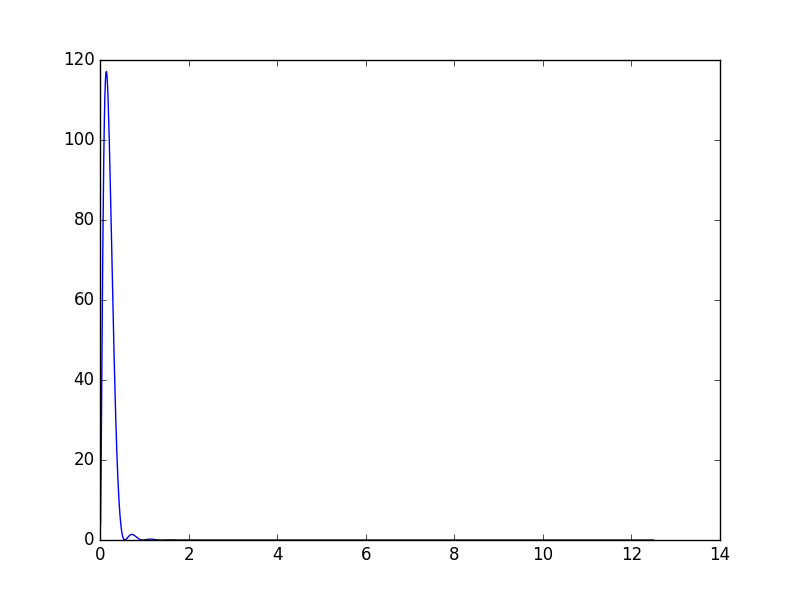
\includegraphics[scale=0.5]{graf.png}
 \caption{\emph{$ \frac{1}{k^5}(ln(1+11.14k))^2 
(1+18.5k + 5880k^2+17580k^3 + 1.04 \cdot 10^6 k^4)^{\frac{1}{2}}(sin(8k) - 8 k  cos(8k))^2$ for $k\le 500$}}
\end{figure}

Por el caracter oscilatorio de la función  a integrar 
(ver los gráficos de la funcion en los 2 casos ) en python la estimación para el error absoluto es bastante grande:
para este caso (r=8)
el resultado sale 6935998.100369965 y el error estimado es 177016.13453597017 (que representa casi 2\% del resultado)

$\frac{9 \sigma_8^2 19843}{2\pi^2 262144}  6935998.100369965 = (0.83)^2 \implies \sigma_8^2 = 2.87784 \cdot 10^{-6}$

para r = 10 (en unidades $h^{-1}Mpc$):

\begin{figure}[H]
 \centering
 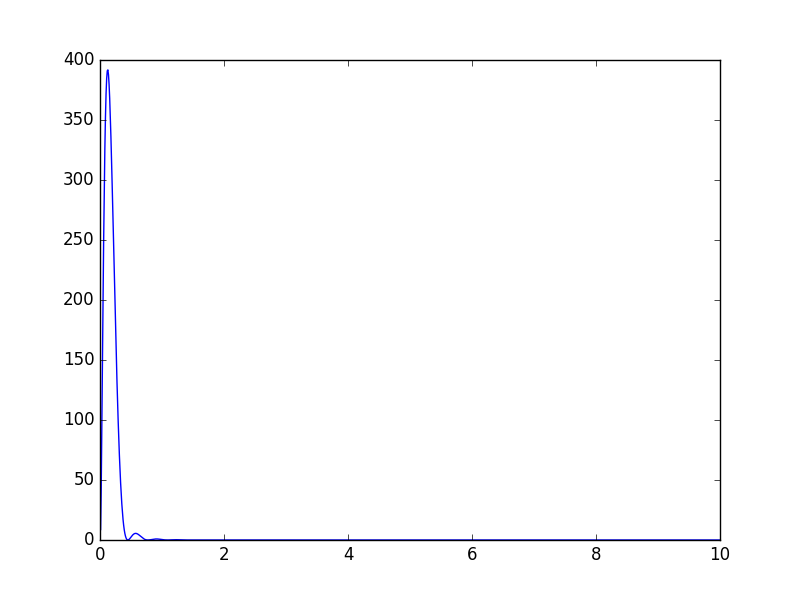
\includegraphics[scale=0.5]{graf2.png}
 \caption{\emph{$ \frac{1}{k^5}(ln(1+11.14k))^2 
(1+18.5k + 5880k^2+17580k^3 + 1.04 \cdot 10^6 k^4)^{\frac{1}{2}}(sin(10k) - 10 k  cos(10k))^2$ for $k\le 500$}}
\end{figure}

el resultado de la integral sale 18504610.63846305 con un error absoluto estimado  13832104.614861604 (casi 74\%)

$<{\delta_r}^2> = \frac{9 \cdot  2.87784 \cdot 10^{-6} \cdot 19843 }{2\pi^2 10^6} 18504610.63846305 = 0.4818$

para r = 30 (en unidades $h^{-1}Mpc$):

\begin{figure}[H]
 \centering
 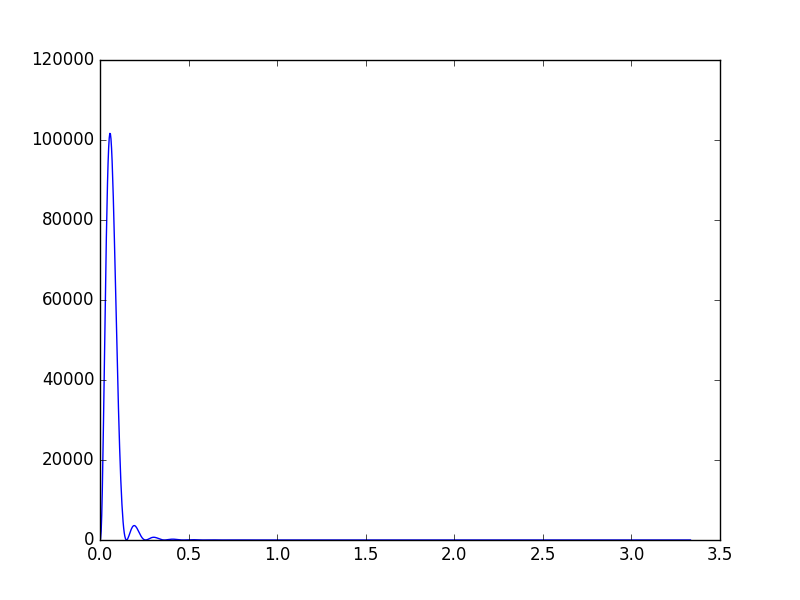
\includegraphics[scale=0.5]{graf3.png}
 \caption{\emph{$ \frac{1}{k^5}(ln(1+11.14k))^2 
(1+18.5k + 5880k^2+17580k^3 + 1.04 \cdot 10^6 k^4)^{\frac{1}{2}}(sin(30k) - 10 k  cos(30k))^2$ for $k\le 500$}}
\end{figure}

el resultado de la integral sale 267972584.74904612 y el error medio abs est es 57299383.581828624 = 21\%

$<{\delta_r}^2> = \frac{9 \cdot  2.87784 \cdot 10^{-6} \cdot 19843 }{2\pi^2 10^6} 267972584.74904612 = 6.97713$


\paragraph{5}

solución general con A, B constantes:

$\delta = A t - \frac{B}{t}$

$\implies \dot \delta = A + \frac{B}{t^2}$

condiciones iniciales $\delta_0=\delta(t=t_0) $ y $\dot\delta_0 = \dot\delta(t=t_0)$

Consideramos solo la situación $\delta_0 = 0$ y $\dot\delta_0 \neq 0$ (la situación $\delta_0 \neq 0$ y $\dot\delta_0 = 0$ 
no es una condición inicial real porque no puede haber una fluctuación sin que haya un cambio)

$\implies A t_0 = \frac{B}{t_0} \implies B = A t_0^2$

$\implies \dot\delta_0 = A + \frac{1}{t_0^2} A t_0^2 = 2 A \implies A = \frac{1}{2} \dot\delta_0$

Consideramos ahora solo el modo creciente:

$\delta = A t$

$\dot \delta = A \implies \delta = \dot\delta t \implies \delta_0 = \dot\delta_0 t_0$

$\delta = A t= \frac{1}{2} \dot\delta_0 t= \frac{1}{2}\delta_0 \frac{t}{t_0}$

universo dominado por radiación $\implies t \propto a^2$

si definimos el factor de crecimiento: $D(a) = a^2$
 
$\delta = \frac{1}{2} \delta_{0} \frac{D(a)}{D(a_{0})} $ 

\end{document}
